\section*{Problem No.2} \label{sec:prob2}

\paragraph{Part b:}  The \emph{not-a-knot} boundary condition requires that $S^{\prime \prime \prime}(x)$ to be continuous at $x_{1}$ and $x_{n-1}$. Thus, the first boundary conditions can be written as 
\[
S^{\prime \prime \prime}_{0}(x_{1}) =  S^{\prime \prime \prime}_{1}(x_{1})
\]
Since we have $d_{j} = \frac{c_{j+1}-c_{j}}{3h_{j}}$ and $S^{\prime \prime \prime}_j = 6d_{j}$, we get
\[
\frac{c_{1}-c_{0}}{3h_{0}} = \frac{c_{2}-c_{1}}{3h_{1}}\\
\]

\begin{equation}
h_{1}h_{2}c_{0} - (h_{1}+h_{0})c_{1} + h_{0}c_{2} =0
\label{eq1}
\end{equation}

Following the same steps for the last interval of the spline i.e., $S^{\prime \prime \prime}_{n-2}(x_{n-1}) =  S^{\prime \prime \prime}_{n-1}(x_{n-1})$, we get 
\begin{equation}
h_{n-1}c_{n-2}-(h_{n-2}+h_{n-1})c_{n-1} + h_{n-2}c_{n}=0
\label{eq2}
\end{equation}


\paragraph{Part c:} We can use the two boundary to define two additional equations that complete the system of linear equations being used to solve the spline problem. The system becomes an $n \times n$ system of equations where the inner $n-2 \times n-2$ equations are the same as in \emph{part (a)} cascaded by the first and and last equations from the boundary conditions which deviates the system from being traditional in the first and last row. 

The following code shows the changes that been done to the original code where we extend the tridiagonal matrix by adding the two new equations. Also, appending the natural conditions is removed.  

\begin{lstlisting}
	%%%%%%%%%%%%%%%%%%%%%%%%%%%%%%%%%%%%%%%%%%%%%%%%%%%%%%%%
    %New Conditions for not-a-knot
    A = [zeros(1,n-2) ; A ; zeros(1,n-2)];
    A = [zeros(n,1), A, zeros(n,1)];  
    
    %From the 1st boundary condition 
    A(1,1)=h(2);%c_{0}
    A(1,2)=-h(2)-h(1);%c_{1}
    A(1,3)=h(1);%c_{2}
    
    %From the original equation at j=1
    A(2,1)=h(1);%c_{0}
    A(2,2)=2*(h(1)+h(2));%c_{1}
    A(2,3)=h(2);%c_{2}
    
    %From the original equation at j=n-1
    A(n-1,n-2)=h(n-2); %
    A(n-1,n-1)=2*(h(n-2)+h(n-1));
    A(n-1,n)=h(n-1);
    
    %From the 2nd boundary condition 
    A(n,n-2)=h(n-1); %c_{n-2}
    A(n,n-1)=-h(n-2)-h(n-1);%c_{n-1}
    A(n,n)=h(n-2);%c_{n}
    
    %%% Update the right hand side 
    b =[0;b;0];
    %%%%%%%%%%%%%%%%%%%%%%%%%%%%%%%%%%%%%%%%%%%%%%%%%%%%%%%%
\end{lstlisting}

%We can use the equation given in \emph{(b)} in conjunction with the new boundary conditions to define two additional equations as follows.
%Applying equation in \emph{(b)} on $j=1$, we get
%\[
%\frac{h_{0}}{h_{1}}c_{0} = \frac{2(h_{0}+h_{1})}{h_{1}}c_{1}+c_{2} = \frac{3}{h^{2}_{1}}(a_{2}-a_{1})-%\frac{3}{h_{0}h_{1}}(a_{1}-a_{0})
%\]

%We can subtract this from Equation \ref{eq1} to eliminate $c_{2}$ and we get
%\[
%\left(\frac{h_{0}}{h_{1}} - \frac{h_{1}}{h_{2}}  \right)c_{0} + \left( \frac{2(h_{0}+h_{1})}{h_{1}} + \frac{h_{1}+h_{0}}{h_{0}} \right)c_{1}= \frac{3}{h^{2}_{1}}(a_{2}-a_{1}) - \frac{3}{h_{0}h_{1}}(a_{1}-a_{0})
%\]
%which will be the first equation in our system of linear equations. Doing the same on the interval $n-1$, we can eliminate $c_{n-2}$ and get the last equation of the system as 
%\[
%\left( 2\frac{h_{n-2}+h_{n-1}}{h_{n-2}} + \frac{h_{n-2}+h_{n-1}}{h_{n-1}}  \right) c_{n-1} + \left( \frac{h_{n-1}}{h_{n-2}} - \frac{h_{n-2}}{h_{n-1}}\right)c_{n} = \frac{3}{h_{n-1}h_{n-2}}(a_{n}-a_{n-1}) - \frac{3}{h^{2}_{n-2}}(a_{n-1}-a_{n-2})
%\]


\paragraph{Part d:}
Figure \ref{fig:fig_d} shows the natural and not-a-knot splines for the interpolated function $f(x)=cos(2\pi x)$ along with the ground truth at $x_{j}=j/5$ for $j=0, \cdots, 5$. 

\begin{figure}[H]
 \centering  
   {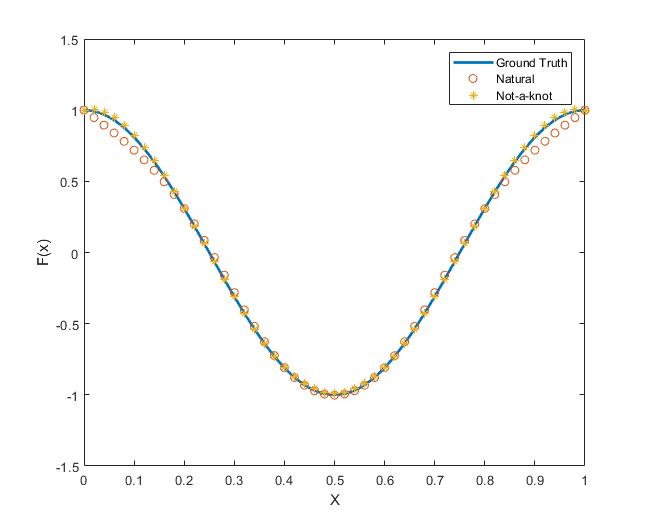
\includegraphics[width=0.98\linewidth]{fig/prob2_d.jpg}}   
  \caption{The natural and not-a-knot spline for $f(x)=cos(2\pi x)$.}
   \label{fig:fig_d}
\end{figure} 

We evaluated the $f(x)$ for both spline at 500 points within [0,1] and the computed the maximum error. For the natural spline it is 0.0952. For the not-a-knot spline it is 0.0181. 

\paragraph{Part e:} Figure \ref{fig:fig_e} shows the natural and not-a-knot splines to interpolate $f(x)=(25x^2+1)^{-1}$ using 21 points between [-1,1].

\begin{figure}[H]
 \centering  
   {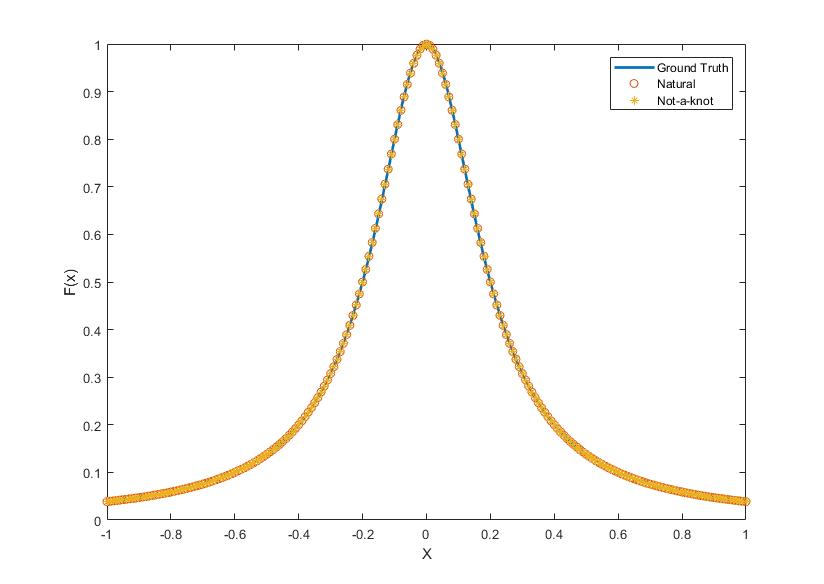
\includegraphics[width=0.98\linewidth]{fig/prob2_e.jpg}}   
  \caption{The natural and not-a-knot spline for $f(x)=(25x^2+1)^{-1}$ .}
   \label{fig:fig_e}
\end{figure} 
Table \ref{tab:part_e} shows the maximum error using increasing number of points. Figure \ref{fig:fig_error} shows the log-log scale plot of the error using using different number of points to interpolate the same function. For the not-a-knot spline, the error of order $h^4$ since the slope of the line 4 on the log-log scale. Same order of the error follows of the natural spline up to number of point equal 161. After that the error is of order $h^2$ (slope of the line is 2). 
\begin{figure}[H]
 \centering
\begin{tabular}{ |c || c|c |}
 \hline
\#points  & Natural Spline & Not-a-knot Spline \\ 
  	
  \hhline{|=|=|=|}                           
%   21  & 0.0031827 & 0.0031827	 & 0.1      & 1.0000e-04 \\
%   41  & 2.7797e-04 & 2.7797e-04 & 0.05     & 6.2500e-06 \\
%   81  & 1.6107e-05 & 1.6107e-05 & 0.025    & 3.9063e-07 \\
%   161 & 1.6142e-06 & 9.6744e-07 & 0.0125   & 2.4414e-08 \\
%   321 & 4.0366e-07 & 5.9822e-08 & 0.00625  & 1.5259e-09 \\
%   641 & 1.0092e-07 & 3.7287e-09 & 0.003125 & 9.5367e-15 \\
   21  & 0.0031827    & 0.0031827	 \\
   41  & 2.7797e-04   & 2.7797e-04 \\
   81  & 1.6107e-05   & 1.6107e-05 \\
   161 & 1.6142e-06   & 9.6744e-07 \\
   321 & 4.0366e-07   & 5.9822e-08 \\
   641 & 1.0092e-07   & 3.7287e-09 \\   
   1281 & 2.5231e-08  & 2.3288e-10\\ 
 \hline
\end{tabular} 
  \caption{The error of both the natural and not-a-knot spline interpolating $f(x)=(25x^2+1)^{-1}$ between [-1,1]. }
   \label{tab:part_e}
\end{figure}


\begin{figure}[H]
 \centering  
   {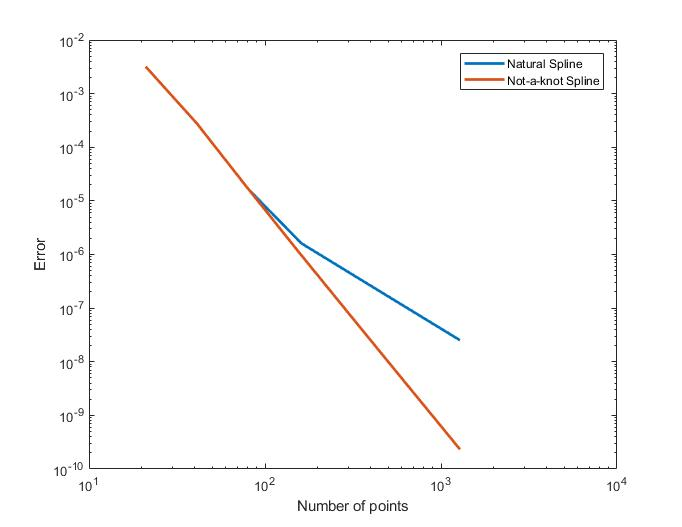
\includegraphics[width=0.9\linewidth]{fig/prob2_error.jpg}}   
  \caption{The log-log plot for the error of spline used to interpolate  $f(x)=(25x^2+1)^{-1}$ using different number of points .}
   \label{fig:fig_error}
\end{figure} 
